%! Author = evandro
%! Date = 13/02/21

% Preamble
\providecommand{\report}{..}
\documentclass[../main.tex]{subfiles}

\begin{document}
    \chapter{Analisi delle performance}\label{ch:analisi-delle-performance}

    La soluzione per via analitica del problema è impraticabile considerata la natura del
    modello utilizzato. I fattori principali che impediscono l’utilizzo di tecniche analitiche
    sono:
    \begin{itemize}
        \item violazione della \textit{service center flow balance}: le perdite non assicurano un ugual numero di arrivi
        \item e completamenti ad ogni stazione.
        \item violazione della \textit{device homogeneity property}: l'utilizzo di code con capacità limitata non
        rispetta questa assunzione.
    \end{itemize}
    Dunque il modello non è separabile, non si possono utilizzare tecniche come la MVA (che
    richiederebbe anche un solo server per stazione); si è deciso di procedere
    con la simulazione a eventi discreti di JMT e con lo strumento \textit{what-if analysis}.


    \section{Approccio utilizzato}\label{sec:approccio-utilizzato}

    \subsection{Analisi dei dati a disposizione}\label{subsec:analisi-dei-dati-a-disposizione}
    Ispezionando i dati a disposizione [\ref{tab:tempo-richiesto-da-ogni-risorsa-per-tipo-di-richiesta}],
    [\ref{tab:set di parametri}, si nota che la classe più popolosa presente nel sistema sono i programmi di
    collaborazione(B). La stazione \textit{application server} ha un \textit{service time} medio per la suddetta classe
    di 120\textit{ms}, maggior valore tra i \textit{service times}.
    Dunque ci aspettiamo che la stazione \textit{application server} abbia bisogno di un maggior numero di repliche
    rispetto le altre due stazione.
    Un ragionamento simile può essere condotto per la stazione \textit{database} rispetto la stazione
    \textit{web server}.
    Tali considerazioni però non tengono conto della lunghezza delle code di ogni stazione che incide in modo
    determinante sulle performance di un sistema.
    Per quanto riguarda la topologia del modello, la stazione con il \textit{throughput} minore influenza le
    stazioni successive ed essendo il modello "circolare", incide sulle altre due stazioni.

    \subsection{Modus operandi}\label{subsec:modus-operandi}
    L'analisi del modello è stata condotta partendo da una configurazione base rispetto al numero di repliche per ogni
    stazioni di coda: \textit{web server}, \textit{application server}, \textit{database}. Ognuna ha inizialmente una
    sola replica.
    Lo step successivo è stato quello di individuare la stazione che agiva da collo di bottiglia per il sistema e di
    aumentarne il numero di repliche.
    Per individuare il collo di bottiglia si è preso in considerazione l'utilizzo di ogni stazione, il valore medio più
    elevato decreta a quale stazione aumentare di uno il numero di repliche.
    Nell'aumentare il numero di repliche, si è anche aggiornato la capacità complessiva della stazione.
    \footnote{\textit{JSIMgrapf} richiede di definire la capacità di una stazione di coda come somma di \textit{jobs} in
    coda e \textit{jobs} che sono processati.}
    L'obiettivo è di avere il \textit{response time} del sistema al di sotto dei 2 \textit{sec}, per cui questi passaggi
    sono stati ripetuti fino al raggiungimento di tale obiettivo.


    \section{Soluzioni ottenute}\label{sec:soluzioni-ottenute}
    In tutte le soluzioni ottenute, gli indici analizzati sono arrivati a convergenza. per ognuno di essi l'intervallo
    di confidenza è pari a 0,99 mentrre l'errore relativo è del 3\%.
    \newline
    Applicando quando detto nella sezione [\ref{subsec:modus-operandi}], la prima configurazione a raggiungere
    l'obiettivo è:
    \begin{table}[h]
        \centering
        \begin{tabular}{|l|c|l|c|l|c}
            \hline
            & \textbf{Utilizzo medio} & \textbf{Utilizzo massimo} & \textbf{numero di repliche (C)}  \\ [0.5ex]
            \hline
            \textbf{WS} & 0.6788                  & 0.6949                    & 1                               \\
            \textbf{AS} & 0,9990                  & 1.0117                    & 7                               \\
            \textbf{DB} & 0.8782                  & 0.8992                    & 4                               \\
            \hline
        \end{tabular}
        \caption{numero di repliche e utilizzo per ogni stazione coda presente nel sistema, soluzione 1.}
        \label{tab:valori-soluzione-1-del-problema}
    \end{table}

    Con questa configurazione [\ref{tab:valori-soluzione-1-del-problema}], si ottiene un \textit{response time} medio del
    sitema pari a 1999,92 \textit{ms}.
    Sebbene riesca ad essere sotto i 2 \textit{sec} richiesti dal progetto, analizzando il valore massimo, esso è pari a
    2017,92 \textit{ms}, non abbastanza da soddisfare le richeiste del prolema.
    Per avere un picco massimo del \textit{response time} del sistema sotto i 2 \textit{sec}, bisogna aggiungere un
    ulteriore replica alla stazione del \textit{application server}.
    \newline
    La nuova configurazione raggiunta:

    \begin{table}[h]
        \centering
        \begin{tabular}{|l|c|l|c|l|c}
            \hline
            & \textbf{Utilizzo medio} & \textbf{Utilizzo massimo} & \textbf{numero di repliche (C)}  \\ [0.5ex]
            \hline
            \textbf{WS} & 0.7741                  & 0.7959                    & 1                               \\
            \textbf{AS} & 0,9704                  & 1.0067                    & 8                               \\
            \textbf{DB} & 0.9868                  & 1.0041                    & 4                               \\
            \hline
        \end{tabular}
        \caption{numero di repliche e utilizzo per ogni stazione coda presente nel sistema, soluzione 2.}
        \label{tab:valori-soluzione-2-del-problema}
    \end{table}

    Con questa nuova configurazione [\ref{tab:valori-soluzione-2-del-problema}], si ottiene un \textit{response time}
    medio del sistema pari a 1704,9896 \textit{ms}; mentre il massimo valore è pari a 1747,1874 \textit{ms}.
    Ambedue i valori sono al di sotto del valore richiesto.


    \section{\textit{What if} delle soluzioni ottenute}\label{sec:what-if-analysis}

    \subsection{Soluzione 1}\label{subsec:soluzione 1}
    Per l'analisi delle soluzioni ottenute, si è incrementata la popolazione classe programmi di collaborazione (B) da
    un valore iniziale di 50 fino ad un valore finale di 110. Tali valori sono stati scelti prendendo in considearazione
    la reale popolazione della classe programmi di collaborazione (B): 100.
    Questa classe risulta essere la più presente per cui è ragionevole analizzare il comportamento del sistema rispetto
    le sue variazioni.
    \begin{figure}[H]
        \centering
        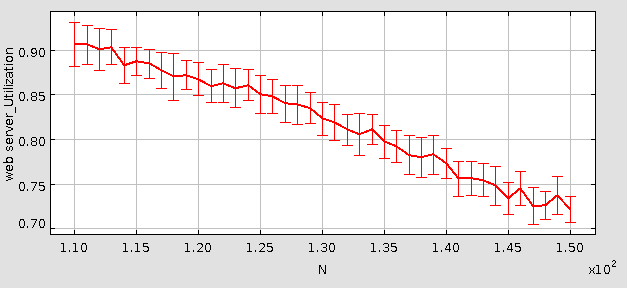
\includegraphics[scale = 0.6]{assets/u_ws_174.png}\\
        \caption[\textit{Utilizzo} della stazione \textit{web server}]{Utilizzo della stazione \textit{web server} al
        variare di N\textsubscript{B}.}
        \label{fig:utilizzo-ws}
    \end{figure}
    Il grafico mostra una riduzione del utilizzo medio del \textit{web server}, ciò è dovuto alla presenza di un collo
    di bottiglia nel sistema. Il \textit{throughput} di tale stazione incide anche sulle altre stazione limitandone, tra
    le altre cose anche l'utilizzo.

    \begin{figure}[H]
        \centering
        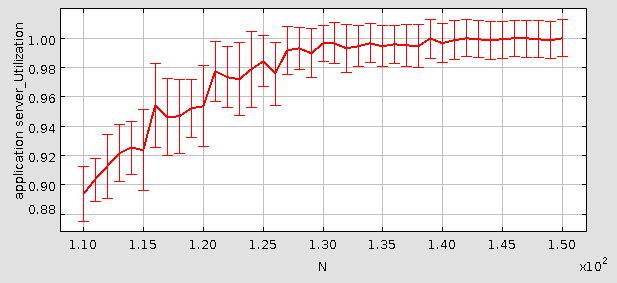
\includegraphics[scale = 0.6]{assets/u_as_174.png}\\
        \caption[\textit{Utilizzo} della stazione \textit{application server}]{Utilizzo della stazione \textit{
            application server} al variare di N\textsubscript{B}.}
        \label{fig:utilizzo-as}
    \end{figure}
    Il grafico mostra un andamento opposta al precedente grafico [\ref{fig:utilizzo-ws}]; è evidente come l'
    \textit{application server} rappresenti il bottleneck di tale sistema e il suo throughput limitato, limiti anche le
    altre risorse del sistema. L'utilizzo medio infatti parte gia da valori elevati (0.9) per arrivare a circa 1
    \begin{figure}[H]
        \centering
        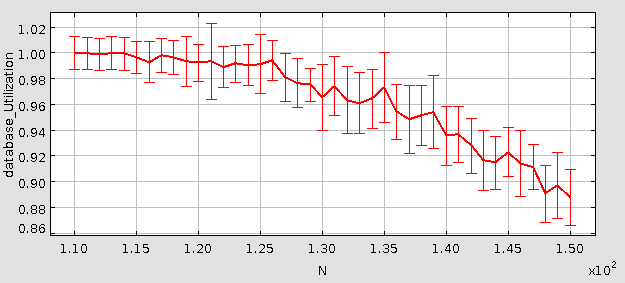
\includegraphics[scale = 0.6]{assets/u_db_174.png}\\
        \caption[\textit{Utilizzo} della stazione \textit{database}]{Utilizzo della stazione \textit{
            databse} al variare di N\textsubscript{B}.}
        \label{fig:utilizzo-db}
    \end{figure}
    Il grafico ha un andamento simile al primo grafico mostrato [\ref{fig:utilizzo-ws}], per cui
    considerazioni a quelle fatte per il \textit{web server} possono essere ripetute anche per il \textit{database}.






\end{document}